\section{The Idea of a Linear Transformation}                                               

\begin{frame}[t]{The Idea of a Linear Transformation: Rules}
    \begin{itemize}
        \item A linear transformation $T$ takes vectors $v$ to vectors $T(v)$
            $\rightarrow$ Linear map
        \item A transformation $T$ follows the same idea as a function.
        \item Linearity requires:
            \begin{itemize}
                \item Rule \#1 - additivity / operation of addition
                  \begin{block}{}
                     \begin{equation*}
                         T(\textbf{v}+\textbf{w}) = T(\textbf{v}) + T(\textbf{w})
                     \end{equation*}
                  \end{block}
                \item Rule \#2 - operation of scalar multiplication
                  \begin{block}{}
                     \begin{equation*}
                         T(c\textbf{v}+d\textbf{w}) = cT(\textbf{v}) +
                         dT(\textbf{w})
                     \end{equation*}
                  \end{block}
            \end{itemize}
    \end{itemize}
\end{frame}

\begin{frame}[t]{The Idea of a Linear Transformation: Rules}
    \begin{columns}[t]
    \begin{column}{0.5\textwidth}
    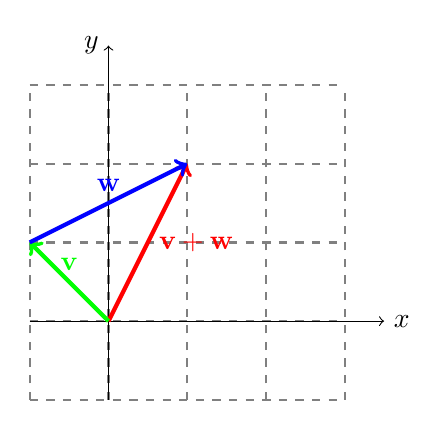
\begin{tikzpicture}[domain=0:2]
        \draw[thick, color=gray, step=1cm,dashed] (-1,-1) grid(3,3);
        \draw[->] (-1,0) -- (3.5,0) node[right] {$x$};
        \draw[->] (0,-1) -- (0,3.5) node[left] {$y$};
        \draw[->, red, line width=1.5pt] (0,0) -- (1,2) node[midway, right]
        {$\textbf{v}+\textbf{w}$};
        \draw[->, green, line width=1.5pt] (0,0) -- (-1,1)
        node[midway,above]{$\textbf{v}$};
        \draw[->, blue, line width=1.5pt] (-1,1) -- (1,2)
        node[midway,above]{$\textbf{w}$};
    \end{tikzpicture}
     \begin{equation*}
        \underbrace{
        \begin{bmatrix}
            -1 \\
            1
        \end{bmatrix}}_{\textbf{v}}
        +
        \underbrace{
        \begin{bmatrix}
            2 \\
            1
        \end{bmatrix}}_{\textbf{w}}
        =
        \underbrace{
        \begin{bmatrix}
            1 \\
            2
        \end{bmatrix}}_{\textbf{v}+\textbf{w}}
    \end{equation*}
    \end{column}
    \begin{column}{0.5\textwidth}
    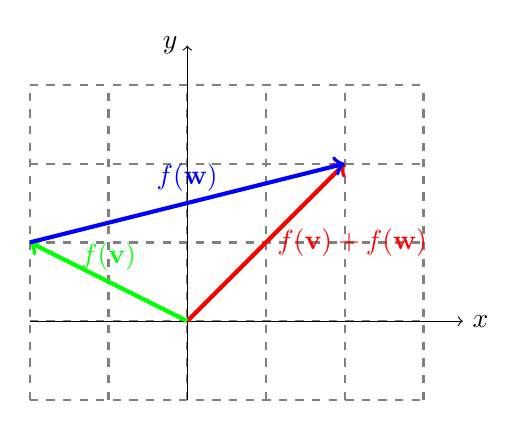
\begin{tikzpicture}[domain=0:2]
        \draw[thick, color=gray, step=1cm,dashed] (-2,-1) grid(3,3);
        \draw[->] (-2,0) -- (3.5,0) node[right] {$x$};
        \draw[->] (0,-1) -- (0,3.5) node[left] {$y$};
        \draw[->, red, line width=1.5pt] (0,0) -- (2,2) node[midway, right]
        {$f(\textbf{v})+f(\textbf{w})$};
        \draw[->, green, line width=1.5pt] (0,0) -- (-2,1)
        node[midway,above]{$f(\textbf{v})$};
        \draw[->, blue, line width=1.5pt] (-2,1) -- (2,2)
        node[midway,above]{$f(\textbf{w})$};
    \end{tikzpicture}
     \begin{equation*}
         f(x,y) = (2x,y)    
     \end{equation*}
       
    \end{column}
    \end{columns}
\end{frame}

\begin{frame}[t]{The Idea of a Linear Transformation: Example in $\textbf{R}^2$}
    \begin{itemize}
        \item In two-dimensional space $\textbf{R}^2$, linear maps are described
            by 2 x 2 matrices (called A).
        \item Example \#1 - rotation by 90 degrees counterclockwise
    \end{itemize}
    \begin{columns}[t]
    \begin{column}{0.5\textwidth}
    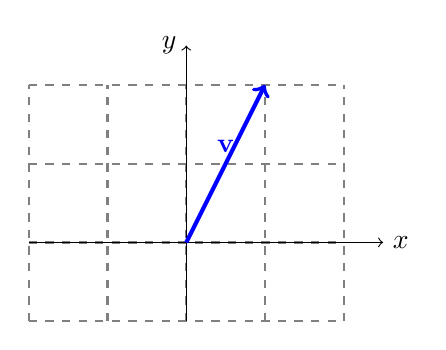
\begin{tikzpicture}[domain=0:2]
        \draw[thick, color=gray, step=1cm,dashed] (-2,-1) grid(2,2);
        \draw[->] (-2,0) -- (2.5,0) node[right] {$x$};
        \draw[->] (0,-1) -- (0,2.5) node[left] {$y$};
        \draw[->, blue, line width=1.5pt] (0,0) -- (1,2)
        node[midway,above]{$\textbf{v}$};
    \end{tikzpicture}
    \end{column}
    \begin{column}{0.5\textwidth}
    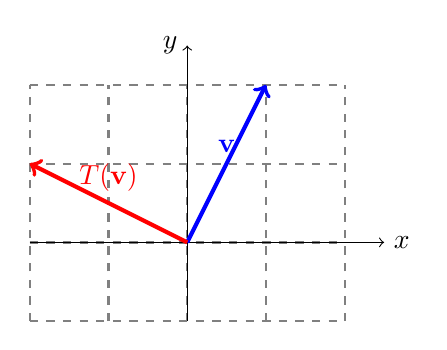
\begin{tikzpicture}[domain=0:2]
        \draw[thick, color=gray, step=1cm,dashed] (-2,-1) grid(2,2);
        \draw[->] (-2,0) -- (2.5,0) node[right] {$x$};
        \draw[->] (0,-1) -- (0,2.5) node[left] {$y$};
        \draw[->, blue, line width=1.5pt] (0,0) -- (1,2)
        node[midway,above]{$\textbf{v}$};
        \draw[->, red, line width=1.5pt] (0,0) -- (-2,1)
        node[midway,above]{$T(\textbf{v})$};
    \end{tikzpicture}
    \end{column}
    \end{columns}

    \begin{equation*}
        \underbrace{
        \begin{bmatrix}
            0 & -1 \\
            1 & 0 
        \end{bmatrix}}_{A}
        \underbrace{
        \begin{bmatrix}
            1 \\
            2
        \end{bmatrix}}_{\textbf{v}}
        =
        \underbrace{
        \begin{bmatrix}
            -2 \\
            1
        \end{bmatrix}}_{T(\textbf{v})}
    \end{equation*}

\end{frame}
